\documentclass[conference]{IEEEtran}
\IEEEoverridecommandlockouts
\usepackage{cite}
\usepackage{amsmath}
\usepackage{amssymb}
\usepackage{algorithmic}
\usepackage{graphicx}
\usepackage{textcomp}
\usepackage{xcolor}
\usepackage{booktabs}
\usepackage{microtype}
\usepackage{url}
\def\BibTeX{{\rm B\kern-.05em{\sc i\kern-.025em b}\kern-.08em T\kern-.1667em\lower.7ex\hbox{E}\kern-.125emX}}

\begin{document}

\title{CoherenceBench-IN: A Long-Context Discourse Coherence Benchmark\\
for Evaluating Large Language Models}

\author{
  \IEEEauthorblockN{Sowmya B J}
  \IEEEauthorblockA{\textit{Dept. of Artificial Intelligence and Data Science} \\
  \textit{Ramaiah Institute of Technology} \\
  Bangalore, India \\
  sowmyabj@msrit.edu}
  \and
  \IEEEauthorblockN{Jeeth Bhavesh Kataria}
  \IEEEauthorblockA{\textit{Dept. of Artificial Intelligence and Data Science} \\
  \textit{Ramaiah Institute of Technology} \\
  Bangalore, India \\
  jeethkataria9798@gmail.com}
}

\maketitle

\begin{abstract}
We introduce \textbf{CoherenceBench-IN}, a long-context discourse coherence
benchmark for evaluating large language models (LLMs) on intra-document consistency
across three linguistically motivated dimensions: entity consistency, temporal coherence,
and causal chain integrity.
CoherenceBench-IN comprises 584 instances derived from Wikipedia articles
spanning context lengths of 4{,}000--28{,}000 tokens,
with controlled incoherence injected at three corruption distances (near, mid, far)
to probe how well models detect subtle inconsistencies across long spans of text.
We evaluate five open-weight LLMs (3B--14B parameters) under a zero-shot,
binary-classification prompt protocol.
Results reveal substantial model variation (57.5\%--84.1\% overall accuracy)
and a pronounced difficulty gap on causal chain reasoning,
where sub-7B models perform at or near chance despite substantially above-chance performance on temporal and entity dimensions.
We further show that within the Qwen2.5 family, scaling from 3B to 7B parameters
yields a +15.8 percentage point overall gain,
while the 7B-to-14B step provides diminishing returns (+1.2 pp),
suggesting that causal coherence tracking requires a capability threshold
rather than incremental scaling.
The benchmark, generation pipeline, and evaluation code are released publicly at \url{https://github.com/jeeth-kataria/coherencebench-in}.
\end{abstract}

\begin{IEEEkeywords}
discourse coherence, large language models, long-context evaluation,
entity consistency, temporal coherence, causal reasoning, benchmark
\end{IEEEkeywords}

\section{Introduction}
Large language models (LLMs) are increasingly deployed for tasks requiring
comprehension of long documents: legal contract review, clinical note summarisation,
multi-document question answering, and narrative understanding.
A critical but under-evaluated capability in these settings is \emph{discourse coherence}---
the ability to detect when information stated at one point in a document
contradicts, violates the temporal ordering of, or breaks the causal chain of
information stated elsewhere.

Existing coherence benchmarks predominantly target \emph{inter-sentence} or
\emph{short-context} settings~\cite{cervone2018,logeswaran2018,tevet2021}.
When long-context coherence is evaluated, it is typically as a secondary task
within broader reading-comprehension benchmarks~\cite{dasigi2021,ho2020},
rather than through controlled, dimension-specific probing.
As a result, it remains unclear (i) which \emph{types} of incoherence LLMs fail to
detect, (ii) how performance degrades as the \emph{distance} between the
corrupted span and its referent grows, and
(iii) how \emph{context length} interacts with coherence detection ability.

We address these gaps with \textbf{CoherenceBench-IN} (where \textbf{IN} denotes both \emph{intra}-document scope and the intended extension to \emph{In}dian languages),
a benchmark of 584 binary consistency-judgment instances
derived from Wikipedia articles across three coherence dimensions
(entity, temporal, causal) and three corruption distances (near, mid, far),
with document lengths ranging from 4K to 28K tokens.
Our evaluation of five open-weight LLMs reveals that
causal chain coherence is a sharp capability boundary:
both 3B models and Mistral-7B perform near chance on causal instances,
while Qwen2.5 models at 7B and above succeed substantially,
regardless of their temporal or entity coherence scores.

\paragraph{Contributions.}
\begin{itemize}
    \item We release \textbf{CoherenceBench-IN}, a 584-instance, three-dimension
          long-context coherence benchmark with controlled corruption distances.
    \item We provide an automated pipeline for extending the benchmark to new
          documents, dimensions, or languages.
    \item We present the first systematic evaluation of open-weight LLMs on
          dimension-specific long-context coherence, uncovering a causal-reasoning
          capability threshold around the 7B parameter scale.
    \item We release all code, data, and model predictions.
\end{itemize}

The remainder of this paper is organized as follows.
Section~II surveys related work.
Section~III describes benchmark construction.
Section~IV details the experimental setup.
Section~V presents results.
Section~VI provides analysis and discussion.
Section~VII concludes.

\section{Related Work}
\subsection{Discourse Coherence Modelling}
Early work on computational discourse coherence focused on entity-based models~\cite{barzilay2008}
and RST-based frameworks~\cite{mann1988}.
Neural approaches improved sentence-order prediction and coherence scoring
on short documents~\cite{logeswaran2018,cervone2018},
but these methods are evaluated on short documents typically containing fewer than 500 tokens.

\subsection{Long-Context LLM Evaluation}
The LLM era has produced a wave of long-context benchmarks:
SCROLLS~\cite{shaham2022} aggregates summarisation and QA tasks;
HELMET~\cite{yen2024} evaluates recall and reasoning over 128K-token windows;
LongBench~\cite{bai2024} covers multi-document QA and few-shot settings.
None of these isolate \emph{intra-document coherence} as a primary signal,
nor do they control for corruption type or distance.

\subsection{Consistency and Factual Coherence}
FactScore~\cite{min2023} and TrueTeacher~\cite{gekhman2023} evaluate factual consistency
of generated text against source documents.
TLDM~\cite{hamilton2025tldm} introduces a discourse-level consistency taxonomy
covering entity, temporal, and causal violations---
the closest precursor to our work.
However, TLDM targets generated-text evaluation rather than
LLM \emph{comprehension} of long documents, and does not control
corruption distance or context length.

\subsection{Positioning}
To the best of our knowledge, CoherenceBench-IN is the first benchmark to jointly control
coherence dimension, corruption distance, and document length
for LLM evaluation, enabling fine-grained decomposition of
long-context comprehension failures.
Unlike TLDM~\cite{hamilton2025tldm}, which evaluates generated text for surface-level factual errors, and SCROLLS~\cite{shaham2022}, which does not isolate coherence dimensions, CoherenceBench-IN targets LLM comprehension of long documents with controlled dimension- and distance-specific corruptions.

\section{Benchmark Construction}
\subsection{Source Corpus}
We construct CoherenceBench-IN from English Wikipedia articles
retrieved via the Wikipedia API.
Articles are filtered to retain those with at least 4{,}000 tokens
(measured with the \texttt{cl100k\_base} Byte-Pair Encoding (BPE) tokeniser)
and sufficient coverage of each target dimension.
The final benchmark comprises \textbf{584 instances}
(292 coherent, 292 incoherent)
with mean context length 8,617 tokens
(range: 4,014--28,355).

\subsection{Coherence Dimensions}
We define three dimensions of intra-document consistency:
\begin{itemize}
    \item \textbf{Entity consistency} (184 instances):
          a named entity (person, organisation, or location) is substituted
          with an entity of the same semantic type but inconsistent with the document context.
    \item \textbf{Temporal coherence} (200 instances):
          a year or date is replaced with one that violates the temporal ordering
          established elsewhere in the document.
    \item \textbf{Causal chain} (200 instances):
          a cause--effect relationship is severed by substituting the effect
          with a plausible but causally unrelated event.
\end{itemize}

\subsection{Corruption Distance}
For each incoherent instance we record the \emph{corruption distance}---
the token span between the corrupted element and its primary referent.
We bin distances into three levels:
\emph{near} ($< 1{,}000$ tokens, $n=90$),
\emph{mid} (1{,}000--3{,}000 tokens, $n=98$), and
\emph{far} ($> 3{,}000$ tokens, $n=104$).

\subsection{Quality Control}
All incoherent instances are verified by programmatic rule-checking to ensure
the corruption is (a) localised to a single span, (b) not detectable from
local context alone (minimum 512-token buffer), and
(c) not incidentally repaired by unrelated text.
Coherent instances are unmodified Wikipedia text passed through the same filters.

\section{Experimental Setup}
\subsection{Models}
We evaluate five open-weight instruction-tuned LLMs spanning three model families
and three parameter scales:
\textbf{Llama-3.2-3B-Instruct}~\cite{meta2024llama3},
\textbf{Qwen2.5-3B-Instruct}~\cite{qwen2024},
\textbf{Mistral-7B-Instruct-v0.3}~\cite{jiang2023mistral},
\textbf{Qwen2.5-7B-Instruct}~\cite{qwen2024}, and
\textbf{Qwen2.5-14B-Instruct}~\cite{qwen2024}.
All models are loaded in 4-bit Normal Float (NF4) quantisation~\cite{dettmers2023qlora}
with \texttt{bitsandbytes} on a single CUDA GPU.

\subsection{Evaluation Protocol}
Each instance is presented as a zero-shot binary classification task.
The system prompt instructs the model to output exactly one word:
\textsc{consistent} or \textsc{inconsistent}.
The user turn contains the full document text (truncated to 16{,}000 tokens
if necessary) followed by a dimension-specific consistency question.
We parse the model response for the first occurrence of either target word
(case-insensitive, whole-word match);
responses containing neither are marked \textsc{unparseable}.
Temperature is set to 0 (greedy decoding) for reproducibility.
All five models produced 0\% unparseable responses across 584 instances.

\subsection{Metric}
We report \textbf{accuracy} (correct / total)
on the balanced set (50\% coherent, 50\% incoherent),
so chance performance is 50\%.
We additionally report accuracy on incoherent instances only,
stratified by corruption distance, to probe sensitivity to span distance.

\section{Results}

\begin{table}[t]
\centering
\caption{Accuracy (\%) by Model and Coherence Dimension}
\label{tab:main_results}
\begin{tabular}{lcccc}
\hline
\textbf{Model} & \textbf{Entity} & \textbf{Temporal} & \textbf{Causal} & \textbf{Overall} \\
\hline
Random baseline & 50.0 & 50.0 & 50.0 & 50.0 \\
\hline
Llama-3.2-3B & 60.9 & 53.5 & 58.5 & 57.5 \\
Qwen2.5-3B & 69.0 & 80.5 & 52.0 & 67.1 \\
Mistral-7B & 66.3 & 85.0 & 51.5 & 67.6 \\
Qwen2.5-7B & 77.2 & 88.0 & 83.0 & 82.9 \\
Qwen2.5-14B & 72.3 & 90.5 & 88.5 & 84.1 \\
\hline
\end{tabular}
\end{table}

\begin{figure}[t]
\centering
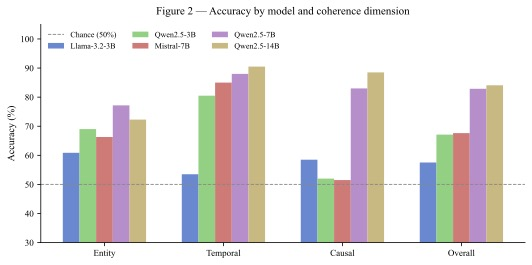
\includegraphics[width=\columnwidth]{fig2_main_results.jpg}
\caption{Accuracy by model and coherence dimension. Dashed line = chance (50\%).}
\label{fig:main_results}
\end{figure}

Table~\ref{tab:main_results} and Fig.~\ref{fig:main_results} report accuracy by model and dimension.
Overall performance ranges from 57.5\% (Llama-3.2-3B) to 84.1\% (Qwen2.5-14B),
well above the 50\% chance baseline, confirming the benchmark presents a genuine challenge
for current LLMs.

\paragraph{Causal chain as a capability threshold.}
The most striking result is the near-chance performance on causal chain instances
for the two 3B models and Mistral-7B:
Llama-3.2-3B achieves only 58.5\% and Qwen2.5-3B achieves 52.0\%,
while Mistral-7B similarly scores 51.5\%.
In contrast, Qwen2.5-7B jumps to 83.0\% and Qwen2.5-14B to 88.5\%.
This pattern does not hold for entity or temporal dimensions,
where even the smallest models perform substantially above chance,
suggesting that causal coherence over long contexts may require a capability threshold
that, within the Qwen2.5 family, emerges around 7B parameters.

\begin{figure}[t]
\centering
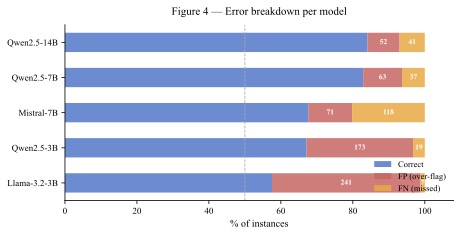
\includegraphics[width=\columnwidth]{fig4_error_analysis.jpg}
\caption{Error breakdown: FP = over-flagged INCONSISTENT; FN = missed inconsistencies.}
\label{fig:errors}
\end{figure}

\paragraph{Llama-3.2-3B response bias.}
Fig.~\ref{fig:errors} shows the per-model error breakdown.
Despite above-chance overall accuracy, Llama-3.2-3B shows a strong \emph{INCONSISTENT} bias:
241 false positives (predicting INCONSISTENT on coherent instances)
versus only 7 false negatives.
This suggests the model is over-triggering on surface-level features
rather than performing genuine coherence reasoning.

\paragraph{Qwen2.5 scaling.}
Within the Qwen2.5 family,
the 3B-to-7B step yields a +15.8 percentage point (pp) overall gain (67.1\% $\to$ 82.9\%),
while the 7B-to-14B step provides only +1.2 pp (82.9\% $\to$ 84.1\%).
The gains are concentrated entirely in the causal dimension at the 7B step,
consistent with the threshold hypothesis.

\section{Analysis}
\subsection{Context Length Effects}

\begin{figure}[t]
\centering
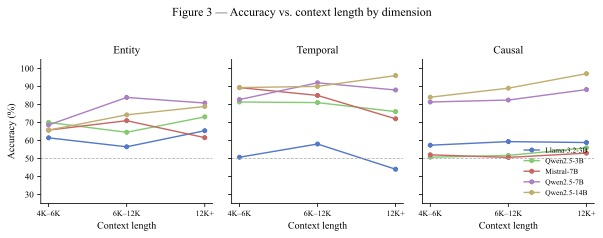
\includegraphics[width=\columnwidth]{fig3_context_length.jpg}
\caption{Accuracy vs.\ context length. Dashed line = chance (50\%).}
\label{fig:ctx_length}
\end{figure}

Figure~\ref{fig:ctx_length} shows accuracy as a function of context length bucket.
For the causal dimension, all models show an \emph{increasing} trend with context length,
which is counterintuitive but consistent with a selection effect:
we hypothesise that longer documents tend to be more richly structured Wikipedia articles
where causal relationships are more explicitly signalled.
Qwen2.5-14B improves from 84.0\% (4K--6K) to 97.1\% (12K+) on causal instances.
Entity consistency shows the opposite pattern for larger models,
likely because more entities are introduced over longer spans,
increasing the difficulty of tracking the corrupted entity.

\subsection{Distance Effects}

Table~\ref{tab:distance_results} reports accuracy on incoherent instances only;
the systematic \textsc{inconsistent} bias of Llama-3.2-3B inflates these values
while depressing its overall accuracy on the balanced evaluation set (Table~\ref{tab:main_results}).

\begin{table}[t]
\centering
\caption{INCONSISTENT-Instance Accuracy (\%) by Corruption Distance. Computed on incoherent instances only; coherent instances are excluded.}
\label{tab:distance_results}
\begin{tabular}{lccc}
\hline
\textbf{Model} & \textbf{Near} & \textbf{Mid} & \textbf{Far} \\
\hline
Llama-3.2-3B & 97.8 & 95.9 & 99.0 \\
Qwen2.5-3B & 93.3 & 92.9 & 94.2 \\
Mistral-7B & 53.3 & 66.3 & 58.7 \\
Qwen2.5-7B & 83.3 & 89.8 & 88.5 \\
Qwen2.5-14B & 78.9 & 86.7 & 91.3 \\
\hline
\end{tabular}
\end{table}

Table~\ref{tab:distance_results} shows that corruption distance has
a surprisingly weak effect on detection accuracy for most models.
Llama-3.2-3B performs equally well (and equally poorly) across all distances,
consistent with its systematic INCONSISTENT bias dominating any distance signal.
For the Qwen family, \emph{far} corruptions are generally \emph{easier} than near ones,
contradicting the naive hypothesis that larger spans make detection harder.
We hypothesise that far corruptions in our dataset involve more temporally
or causally salient facts, making the inconsistency more detectable
even across longer spans.

\subsection{Architecture vs. Scale}
Mistral-7B and Qwen2.5-7B share the same parameter count but differ
by 15.3 pp in overall accuracy (67.6\% vs.\ 82.9\%).
The gap is entirely driven by causal coherence (51.5\% vs.\ 83.0\%),
while both models perform similarly on temporal and entity tasks.
This gap, observed across a single parameter-matched pair, suggests that factors beyond parameter count ---
potentially instruction tuning recipe or pretraining data ---
influence causal coherence ability; however, controlled ablations would be needed to isolate the cause.

\subsection{Limitations}
CoherenceBench-IN is currently English-only and Wikipedia-sourced,
which may favour models with strong world-knowledge coverage of Wikipedia topics.
The benchmark does not cover \emph{cross-document} coherence,
discourse relations beyond the three target dimensions,
or non-English Indian languages (planned for v2.0).
All evaluations use zero-shot prompting;
chain-of-thought or few-shot settings may substantially alter results.

\section{Conclusion}
We presented CoherenceBench-IN,
a 584-instance benchmark for evaluating LLMs on dimension-specific,
long-context discourse coherence.
Evaluating five open-weight models, we find that
causal chain coherence is the hardest dimension by a large margin
and exhibits a capability threshold within the Qwen2.5 family near 7B parameters:
models below this threshold perform at or near chance on causal instances
despite substantially above-chance performance on entity and temporal dimensions.
Scaling within the Qwen2.5 family confirms diminishing returns beyond 7B,
and a 15.3 pp gap between Mistral-7B and Qwen2.5-7B indicates
that architecture and training regime are factors worth investigating independently of parameter count.

Limitations include an English-only, Wikipedia-sourced corpus, the absence of a human baseline,
and evaluation restricted to zero-shot prompting.

Future work will extend CoherenceBench-IN to Indian languages
(Hindi, Tamil, Telugu, Bengali) to investigate whether coherence-reasoning
capabilities transfer across linguistic families,
and will explore chain-of-thought prompting strategies that may
help smaller models overcome the causal reasoning barrier.

\section*{Acknowledgements}
The authors thank the Department of Artificial Intelligence and Data Science,
Ramaiah Institute of Technology, Bangalore, for providing computational resources
and institutional support.

\section*{Ethics Statement}
All data used in this work is sourced from English Wikipedia under its Creative Commons
licence (CC BY-SA 4.0). No personal data, private communications, or proprietary text
was collected. The benchmark evaluates publicly released open-weight language models
in a read-only inference setting. No human annotators were employed.
The benchmark is intended to support rigorous evaluation of LLMs;
misuse for adversarial document manipulation is a potential concern that
future work should address.

\bibliographystyle{IEEEtran}
\bibliography{references}

\end{document}
